\documentclass[9pt]{beamer}

\usepackage[T1]{fontenc}
\usepackage[utf8]{inputenc}
\usepackage[english]{babel}
\usepackage{graphicx}
\usepackage{listings}
\usepackage{tikz}
\usepackage{rotating}

\usetikzlibrary{arrows,calc,shapes,positioning}

\usepackage{amsmath}
\usepackage{listings}

% FU logo
\pgfdeclareimage[height=0.9cm]{university-logo}{res/fu-logo}
\logo{\pgfuseimage{university-logo}}
% title page logo
%\newcommand{\titleimage}[1]{\pgfdeclareimage[height=2.92cm]{title-image}{#1}}
%\titlegraphic{\pgfuseimage{title-image}}

% remove sidebars
\setbeamersize{text margin right=3.5mm, text margin left=7.5mm}
\setbeamersize{sidebar width left=0cm, sidebar width right=0mm}
\setbeamertemplate{sidebar right}{}
\setbeamertemplate{sidebar left}{}

%%% colors
\definecolor{text-grey}{rgb}{0.45, 0.45, 0.45}
\definecolor{bg-grey}{rgb}{0.66, 0.65, 0.60}
\definecolor{fu-blue}{RGB}{0, 51, 102}
\definecolor{fu-green}{RGB}{153, 204, 0}
\definecolor{fu-red}{RGB}{204, 0, 0}

\usecolortheme{lily}
\setbeamercolor*{normal text}{fg=black,bg=white}
\setbeamercolor*{alerted text}{fg=fu-red}
\setbeamercolor*{example text}{fg=fu-green}
\setbeamercolor*{structure}{fg=fu-blue}

\setbeamercolor*{block title}{fg=white,bg=black!50}
\setbeamercolor*{block title alerted}{fg=white,bg=black!50}
\setbeamercolor*{block title example}{fg=white,bg=black!50}

\setbeamercolor*{block body}{bg=black!10}
\setbeamercolor*{block body alerted}{bg=black!10}
\setbeamercolor*{block body example}{bg=black!10}

\setbeamercolor{bibliography entry author}{fg=fu-blue}
\setbeamercolor{bibliography entry journal}{fg=text-grey}

\setbeamercolor{item}{fg=fu-blue}
%%% end colors

%%% title page
\setbeamertemplate{title page}{
    % title image
    \vskip30pt
    \begin{minipage}{11.6cm}
        \hspace{-0.5cm}\inserttitlegraphic
    \end{minipage}

    % title and author
    \vskip16pt
    \parbox[top][1.35cm][c]{11cm}{
        \color{black}
        \inserttitle\\
        \small\insertsubtitle
    }
    \vskip12pt
    \parbox[top][1.35cm][c]{11cm}{
		\color{text-grey}
        \small\insertauthor\\
        \insertinstitute\\[3mm]
        \insertdate
    }
}
%%% end title page

%%% frame title
\setbeamertemplate{frametitle}{
    \vskip-30pt
    \color{text-grey}
    \large
    \begin{minipage}[b][23pt]{80.5mm}
        \flushleft\insertframetitle
    \end{minipage}
}
%%% end frame title

%%% header
\setbeamertemplate{headline}{
    \vskip5pt\hfill\insertlogo\hspace{3.5mm}
    \vskip5pt\color{fu-blue}\rule{\textwidth}{0.4pt}
}
%%% end header

%%% footer
\newcommand{\footlinetext}{
    \insertshortinstitute,
    \insertshorttitle,
    \insertshortdate
}

\setbeamertemplate{footline}{
    \vskip5pt\color{fu-blue}\rule{\textwidth}{0.4pt}\\
    \vskip3pt
    \makebox[123mm]{
        \hspace{7.5mm}
        \color{fu-blue}\footlinetext
        \hfill \insertframenumber
    }
    \vskip3pt
}
%%% end footer

%%% listings
\lstset{
    extendedchars=true,
    showstringspaces=false,
    basicstyle=\footnotesize\sffamily,
    tabsize=2,
    breaklines=true,
    breakindent=10pt,
    frame=l,
    columns=fullflexible,
    language=C,
    literate={ä}{{\"a}}1 {ö}{{\"o}}1 {ü}{{\"u}}1 {Ä}{{\"A}}1 {Ö}{{\"O}}1 {Ü}{{\"U}}1 {ß}{\ss}1
}
%%% end listings


%\titleimage{ }

\title{Erweiterungen für VAST}
\subtitle{Importer, Middleware und Web-Applikation}
\author{Samir Al-Sheikh, Andreas Reuter, Fabrice Ryba, Robert Schmidt}
\institute[FU Berlin]{Freie Universität Berlin}
\date[]{Softwareprojekt Technische Informatik, SS 2015}

\renewcommand{\footlinetext}{\insertshorttitle, \insertshortauthor} % \insertshortinstitute, 

\AtBeginSection[]
{
  \begin{frame}<beamer>{Gliederung}
    \tableofcontents[currentsection]
  \end{frame}
}


\begin{document}

\begin{frame}
    \titlepage
\end{frame}

\begin{frame}{Gliederung}
  \tableofcontents
\end{frame}


\section{Motivation}

\subsection{BGP und BGP-Hijacking}

\begin{frame}{BGP Funktionsweise}{}
	\begin{center}
		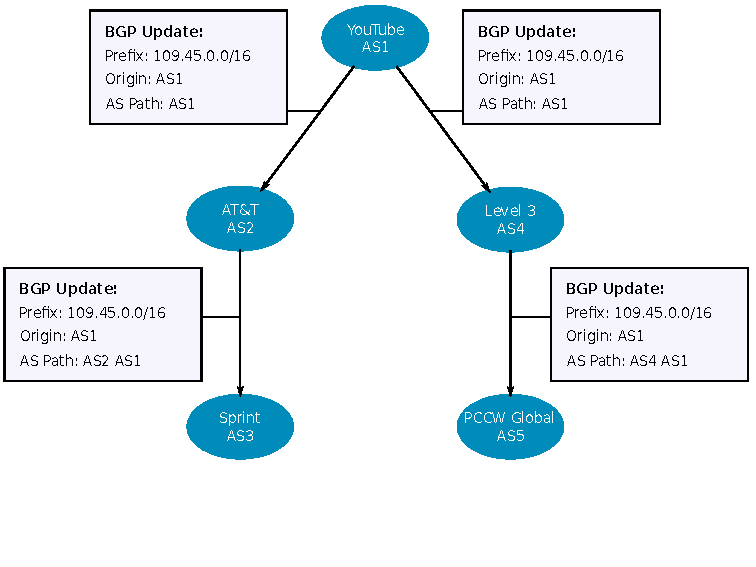
\includegraphics[width=1.0\textwidth]{res/bgp_propagation.pdf}
	\end{center}
\end{frame}

\begin{frame}{BGP Hijacking}{}
	\begin{center}
		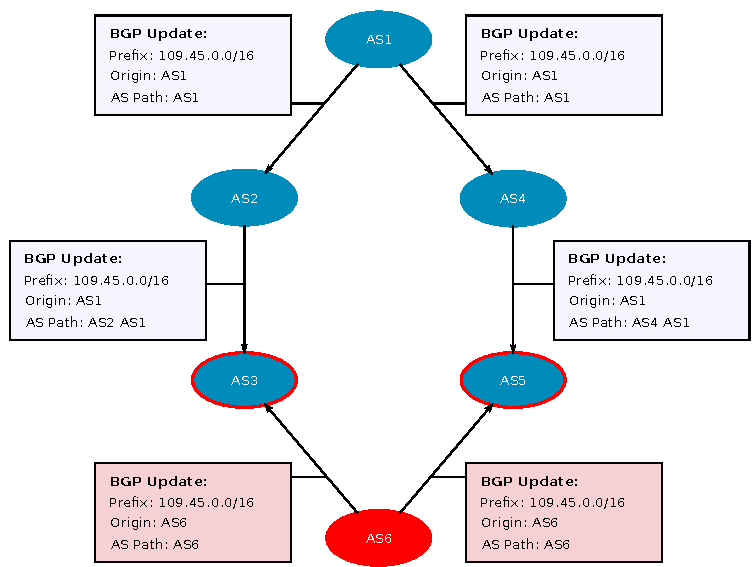
\includegraphics[width=0.85\textwidth]{res/prefix_hijack.pdf}
	\end{center}
\end{frame}

\subsection{VAST}

\begin{frame}{VAST = Visibility Across Space and Time}{}
	\begin{itemize}
		\item bietet eine sehr schnelle Durchsuchung von Massendaten
		\item ...
	\end{itemize}
\end{frame}


\section{Ziele}

\begin{frame}{Motivation und Ziele}{}
	\begin{itemize}
		\item bisheriger BGP-Importer liest nur Text-Format ein --> langsam bei vielen Dateien
		\item Erweiterung des BGP-Importers, um gängige Binär-Formate nativ einzulesen
		\item User-Interface bisher nur über Konsole
		\item Erweiterung um Graphische Web-Oberfläche zur Datenvisualisierung
		\item Dazu:
		\begin{itemize}
			\item Entwicklung einer REST-Schnittstelle (Middleware)
			\item Entwicklung einer Web-Anwendung für die Analyse von BGP-Daten
		\end{itemize}
	\end{itemize}
\end{frame}

\section{Software-Komponenten}

\begin{frame}{Software-Komponenten}{}
	\begin{center}
		%\includegraphics[width=1.0\textwidth]{res/vast_architecture.pdf}
	\end{center}
\end{frame}

\subsection{Importer}

\begin{frame}{Importer}{}
	...
\end{frame}

\subsection{Middleware}

\begin{frame}{Middleware - Implementierung}{}
	\begin{center}
		%\includegraphics[width=1.0\textwidth]{res/???.pdf}
	\end{center}
\end{frame}

\begin{frame}{Middleware - Stand und Probleme}{}

	heutiger Stand:
	\begin{itemize}
		\item ...
	\end{itemize}

	Probleme:
	\begin{itemize}
		\item ...
	\end{itemize}
	
	nächster Milestone:
	\begin{itemize}
		\item ...
	\end{itemize}

\end{frame}

\subsection{Web-Anwendung}

\begin{frame}{Web-Anwendung}{}
	...
\end{frame}

\section{Demo}

\begin{frame}{Demo}{}
	...
\end{frame}


\end{document}

% vim: ft=tex tw=0
